\documentclass{article}
\usepackage{graphicx}
\usepackage{subcaption}
\usepackage{caption}
\usepackage[utf8]{inputenc}

\begin{document}
\title{Process Analysis}
\author{\textbf{DAT2-A423}\\  
    Søren Madsen\\
    Leo Johannesen Mohr\\
    Theresa Krogh-Walker\\
    Jakob Meldgaard Kjær\\
    Henrik Herbst Sørensen\\
    Mathias Steen Jakobsen\\ 
    Jacob Askløf Svenningsen}
\date{\today}
\maketitle 
\section{Working Within the Group}
As a part of working within the group, we have had various different ways of working together. 
At the beginning when we started writing our problem analysis, each person got a section they had to investigate and write about. 
When the problem analysis was written, we moved on to the development stage. 
In the development stage we did the same as before, but this time split the group up into smaller groups to divide the workload. 
Each group got the task of constructing and finishing the various parts of our programme and documentation thereof. 
With regards to correcting our report, we read the whole report together and came with our individual corrections and helped each other complete the task that way.

Working in this way worked well for us. Not only did we learn how to work individually, but also in smaller groups. 
And to bring the entire project together, working as a whole group on correcting the report, made it certain that everyone was aware of what was written in the report as well as teaching us how to share our knowledge.
One problem we came across as we dealt the various assignments out, was that not everyone had been made clear who had received what assignment. This resulted in some people writing the same thing.

We have also had to try and plan our time effectively. 
This was done by creating a schedule that covered the whole semester. 
However, along the way, we created some smaller deadlines, to help keep us aware that we had deadlines to reach, and creating them and discussing them throughout the project, helped with keeping them fresh in our minds.

In our group contract, we had decided to have one set meeting per week. At this meeting, we would discuss the group's attendance, what has been done, if anyone has discovered anything worthwhile regarding the project, what still needs to be done and what needs correcting. 
At these meetings we would also discuss if there had been any discrepancies within the group. So it gave each member an opportunity to speak up if they had any problems.
We had also agreed to decide when the next meeting would be at these meetings, however, as we saw each other almost every day because of our lectures, this was not necessary.

This weekly meeting gave us a good overview of how the project was going and allowed us to express how we felt regarding the atmosphere in the group room. 

We have not had any extraneous group activities. 
We do not feel as though this has been detrimental to our process.
Another thing that has been different this project, is that we have not held defined breaks. 
This has made working much more flexible, than it would have been if we had set specific times of day to have a break. 
Some group members preferred this more flexible way, as they did not feel so confined when it came to having a break and instead could do so as they felt a need to.

We also tried to coordinate our work so it was more flexible for individual group members. If you wanted to stay at home and work from there, this was no problem. We found out that this was a very effective way of working, as there were no distractions in the group room and we were able to focus on one thing at a time. At the start of the project we quickly found out that we end up distracting each other and work that should not take that long, ended up taking a few hours.

\section{Working with the Supervisor}
At the first supervisor meeting with Kurt we came to the agreement that material should be sent 24 hours in advance, unless otherwise agreed upon. 
We had also agreed on providing the supervisor with an agenda for our meetings, so that there was no confusion on what was to be focused on at the meetings. 
Our original idea was to create a formal agenda, but it ended up with being more of a discussion, where we wrote to Kurt what we had done and what we wanted to discuss at the meeting. 
We feel that this has gone well, as we feel that at every meeting we held with Kurt, we received a lot of information as to how we can improve our work and how to further our project.

\section{Project Management}
\subsection{Group Contract}
At the beginning of the project we created a group contract. 
Everyone in the group was in agreement with the various conditions the contract set at the time of creation. 
Some of the agreements made in this contract are described in the following sections.

\subsection{Project Leader}
For this project we decided to have a project leader, to take control of the group for a week at time. 
This was a role that everyone was supposed to try at some point during the course of the project. 
The project leader role consisted of making sure that the group held concentration and did not get too sidetracked, coordinate meetings and keep in contact with our supervisor. 
Another job the project leader had, was to handle conflicts within the group. 
Another task the project leader had was to update our Trello board.
We realised after the first time someone had tried being group leader, that one week was simply not enough for them to get accustomed to the role of project leader.
Therefore, the number of weeks a group member had to be leader was upped to two.

Not every group member had the same enthusiasm for the role. 
Some were better at taking command than others especially in concern to taking control of the group.
This is something that individuals became aware of as they were in the position.
Neither was there a need for the group manager to discuss problems within the group, as there were no huge issues that we came across that could not be solved within the group room.
The task of updating our Trello board, did not go quite as planned. 
It ended up with it being the person who wrote a summary of any meetings that updated the board.

\subsection{Attendance}
Throughout this semester, we have taken attendance. 
Every time the group had a meeting or a lecture, attendance was taken. 
This was done to ensure that we had concrete details on when a person was present or not. 
If attendance came under 80\%, we had agreed that the person had to talk to the project leader and find out why their attendance had been so poor. 
If attendance came under 65\%, the person in question had to be evicted from the group. 
We thought it necessary to have details of attendance, so that if it did become a problem, we could show the person solid evidence of their absence. 
The reason for taking attendance was based on past experiences of half the members of the group. 
Taking attendance could also lead to some form of motivation for people showing up when meetings are held.
On figure \ref{fig:GraphImage}, we have the general overview of the group's attendance. We can also see when a specific group member has been absent as seen on figure \ref{fig:soerenfravaer}.
An issue that we came upon when starting this project, was taking attendance at the start of the semester, since if a person was absent just two days into the project, their attendance would be incredibly low. 
So something that should have been discussed further, was when we started enforcing the attendance rule. 
This semester, attendance has not been a large issue. 
It is unknown whether it was our attendance taking that did this, or whether it was just the different group members that were more motivated.
We have discussed that even if a group member came down to 65\% it was necessary to discuss further, as not every member of the group feels as though they could do it, and would rather see why attendance had become so poor instead of drawing the line at 65\%, with no exceptions.

\begin{figure}
	\centering
	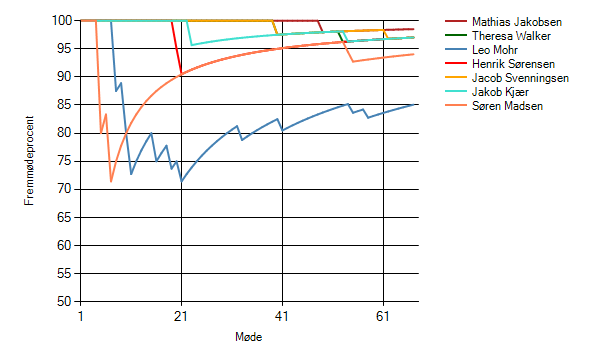
\includegraphics[width=1\textwidth]{figures/GraphImage.png}
	\caption{An oversight of the group's absence}
	\label{fig:GraphImage}
\end{figure}

\begin{figure}
	\centering
	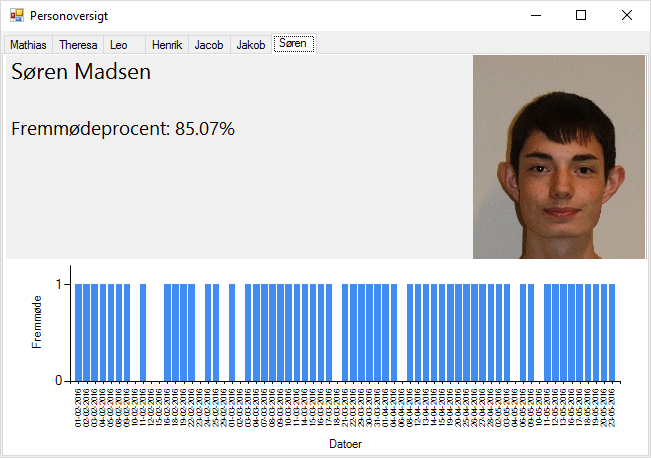
\includegraphics[width=1\textwidth]{figures/soerenfravaer.png}
	\caption{A specific group member's attendance sheet}
	\label{fig:soerenfravaer}
\end{figure}

\section{Learning Process}
In this project, we have used various tools to communicate, share documents and plan upcoming meetings with each other. 
We discussed that we would not use Facebook to communicate with each other to keep forms of communication professional. Another issue with using Facebook, is that not every group member had an account.
Instead, we have used Slack, as seen on figure \ref{fig:slack}, an alternative method of communicating with each other. 
This programme was only used for talking to other group members and sharing relevant information. 
It has been used for sharing relevant information, but also to inform the other group members if they could not be there that day or were delayed. 

We also used a website, Trello, as can be seen on figure \ref{fig:trello}, that allowed us to write and see what our report was missing and when we had meetings. 
Towards the end of this project Trello was almost exclusively used as a way of documenting our meetings and saving the summaries of these meetings, instead of writing parts of the report that are missing. 
This was, instead, done by discussing amongst ourselves at our weekly meetings.
However, it has been a good thing to see all the things that have been completed and things that are missing to help us with our overview of the project.
We could have been much better at using Trello to avoid people writing the same things. This could have been rectified by instead of just writing the assignments on our black boards, write them in Trello, so people could put their names on the assignment that they wished to have.

\begin{figure}
	\centering
	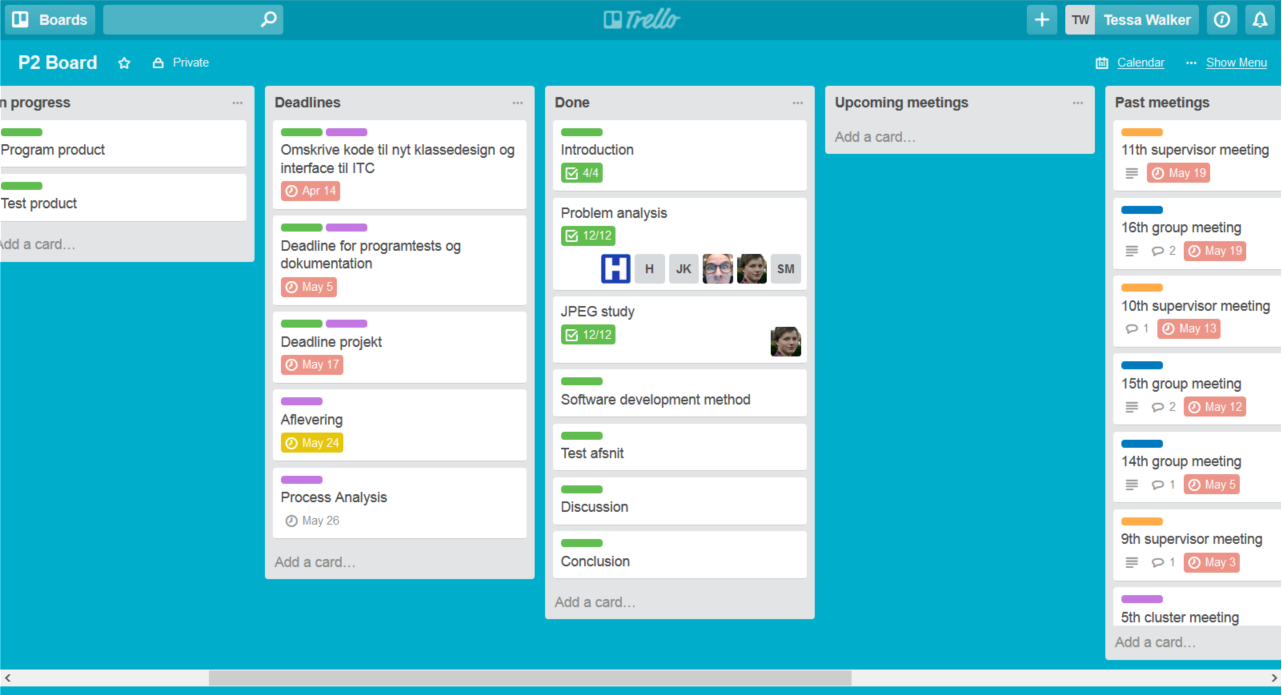
\includegraphics[width=1 \textwidth]{figures/trello.png}
	\caption{A screenshot of our Trello board}
	\label{fig:trello}
\end{figure}

\begin{figure}
	\centering
	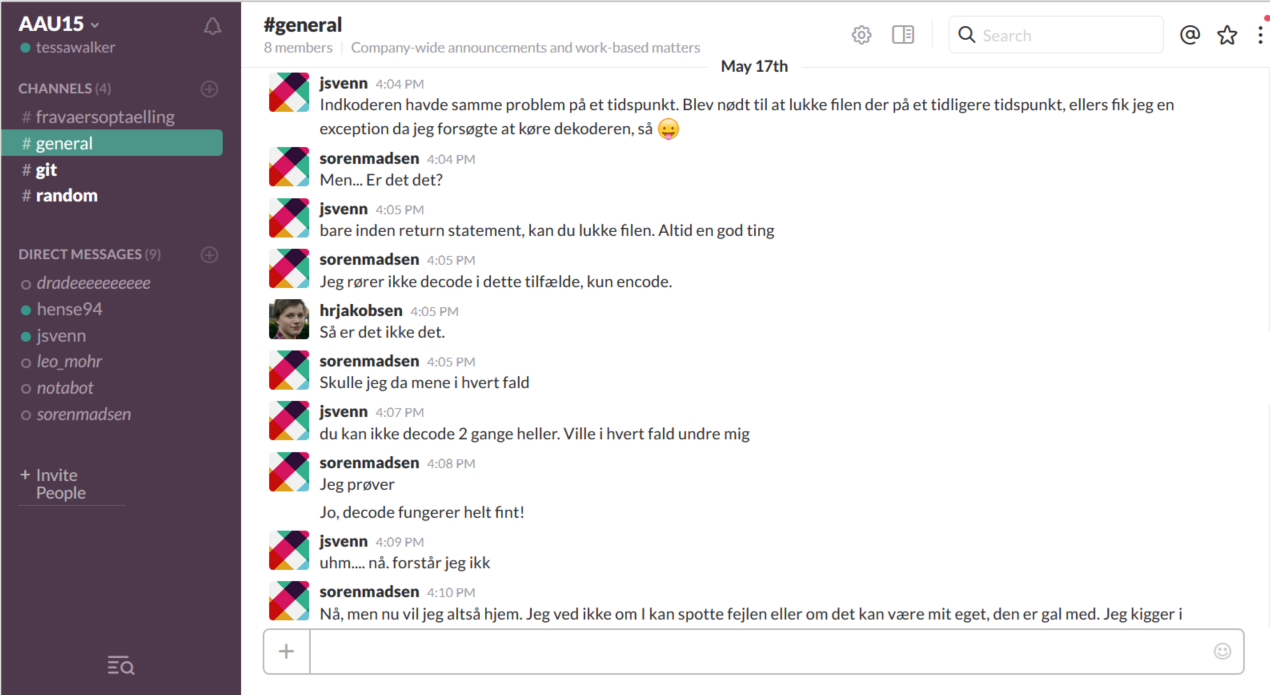
\includegraphics[width=1 \textwidth]{figures/slack.png}
	\caption{A screenshot of our Slack communication}
	\label{fig:slack}
\end{figure}

\begin{figure}
	\centering
	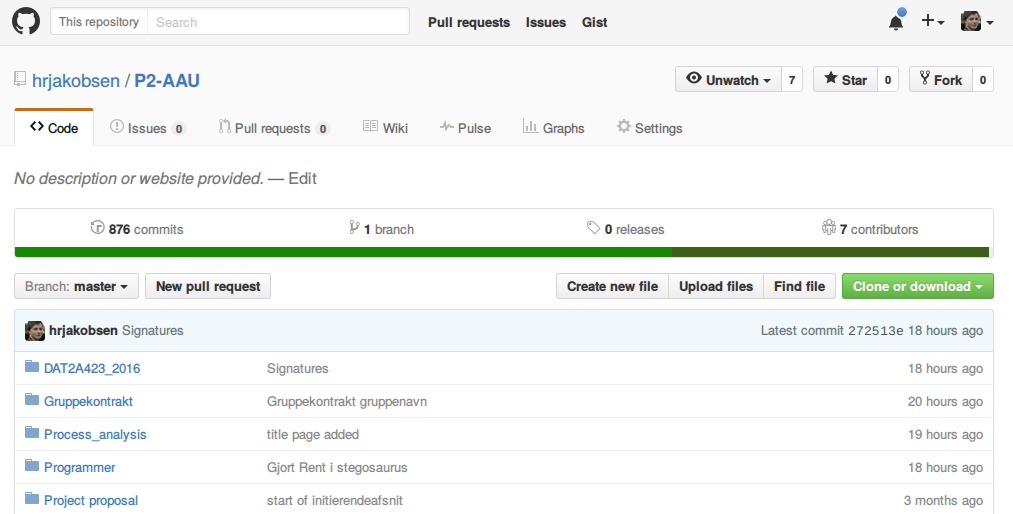
\includegraphics[width=1 \textwidth]{figures/git.png}
	\caption{A screenshot of our GitHub}
	\label{fig:git}
\end{figure}

For sharing documents with each other, we have used Github, as seen on figure \ref{fig:git}.
This has worked well for us. 
An example of this, is being able to revert back to an earlier stage in the project to retrieve code that we needed later in the project. There were some issues with Git, where we have been working in the same files and had some merge conflicts. Fixing these merge conflicts can be quite time-consuming.
However, regarding writing our report, there could have been other options that were just as good, or maybe even better. An option that we have considered is using ShareLaTeX. This would have made it easier for us to correct our report, especially towards the end of the project, as we could all have been in the same documents without any major problems. However, the possibility of ShareLaTeX came late in the project and we already had something that worked reasonably well, so we continued with our use of Git.


\section{Cluster Group}
This project has had a different element to it. We have had to work with two other groups and try and get these groups to work together.
\subsection*{Concerns}
There have been a number of cluster meetings with the groups from Mathematics (MAT) and Internet Technologies and Computer Systems (ITC), and us, Computer Science (DAT), as well as with each group's project supervisors.
In the beginning there was a bit of uncertainty in our group about how the entire process would work, since each group in the cluster had a different curriculum and a different set of requirements to be fulfilled.
Furthermore, we were concerned about the fact that each group had to figure out a part of the whole solution based on the work of others.
Essentially, it sounded like MAT would develop an algorithm as a base for us (the Computer Science group) to use.
DAT would then use this algorithm and develop a class library for the ITC group to use.
ITC would finally use the algorithm and the library in their project.
This would require a lot of time and be largely inefficient, since one step of the process had to be completed before another one could begin, and we only had about four months for the project in total.
It would also mean that ITC would be dependent on DAT, while DAT would be dependent on MAT for their respective projects, and that would not be feasible.
In a similar vein, the point of the cluster group was that each group could benefit from the work of others.
But how could our group benefit from the work of ITC if they were dependent on us? And would MAT gain any benefit from the cluster group at all?

\subsection*{Trying to work together}
There was no real progress in the cluster collaboration during the first weeks, which was expected, as we were all finding out which direction we wanted the project to take.
Everyone was busy learning about steganography and how to use it.
Our group made a fairly trivial programme to embed data into other data using least significant bits, but we could not spend the entire project on that. However, this programme was not completely useless with regards to ITC, as ITC could use it, and it was decided that DAT would deliver either that or whichever better programme that was developed later.

Olav Geil, MAT's advisor, held a lecture on an article about a graph-theoretic approach to steganography.
This proved to be valuable to both us and MAT, as both groups would later decide to use this approach in some form.
DAT and MAT somewhat connected over this, thinking this could be the key to the lacking collaboration.
We were encouraged by the supervisors to collaborate, perhaps letting MAT develop and giving us an efficient algorithm using this approach, while DAT developed a slightly less efficient algorithm for testing purposes until MAT was done with their investigations.
When voicing concern about how MAT would benefit from this, we were told that it could possibly be exciting for them to see their algorithm in action.

To solidify the demise of the cluster project, we realised at a cluster meeting - roughly a month before the final deadline - that DAT and MAT had chosen different paths.
MAT had dedicated their time to make the algorithm presented by Olav Geil as precise as possible, sacrificing efficiency, while DAT were looking for an efficient algorithm where extreme precision had less of a priority.
This meant that MAT and DAT would be of no use to each other, and it was decided that it was the end of the collaboration between DAT and MAT.
ITC would still, however, get a complete steganographic solution to use as a library with select methods exposed, since they had no use for the entire codebase in their project.

\subsection*{Improvements}
We believe that this cluster group work would have turned out a lot better if we had had someone to take control of communication between the groups and make sure that we had all understood what each group was supposed to do. 
We would have preffered having someone, not a part of the cluster groups, to have this project leader role, so they have more of an overview over what each of the groups are doing. We felt that we lacked this overview througout the project due to poor communication.
Often, a couple of weeks would pass before any form of communication happened between the groups. 
If this had not been the case, our collaboration with the other groups might have been more successful. 

If this cluster group had been part of our curriculum, there would have been more motivation for getting the project to work. However, as it was almost optional, it did not seem as important to us, as we were more focused on getting our own projects off the ground, rather than trying to create one larger project across different subjects.
\vspace{12pt}

To summarise, we have these few points:
We will begin with:
\begin{itemize}
\item Using Trello more effectively than we have.
\item Being better at focusing on the task at hand.
\item Trying to use ShareLatex.
\end{itemize}

We will continue to:
\begin{itemize}
\item Keep taking attendance.
\item Share the various tasks amongst group members.
\item Send material to our supervisor not at last minute.
\item Use Slack as our main communication tool.
\item Use Git to share our documents.
\end{itemize}

We will stop with:
\begin{itemize}
\item Using our time ineffectively.
\end{itemize}

\end{document}